\documentclass[a4paper,12pt]{letter}
\usepackage[margin=2.2cm]{geometry}
\usepackage{amsmath,amssymb}
\usepackage{physics}
\usepackage{tikz}
\usepackage{lmodern}

\setlength{\parindent}{0pt}
\setlength{\parskip}{0.6em}

\begin{document}

\begin{center}
\textbf{\huge Nabla Operator and Integral Theorem}
\end{center}


The nabla operator is defined by
$$
\nabla = \left( \pdv{}{x}, \pdv{}{y}, \pdv{}{z} \right).
$$

%------------------------------------------------
\textbf{1. Gradient of a Scalar Field}

Let $\phi(x,y,z)$ be a scalar field. Its gradient is
$$\nabla \phi =
\left(
\pdv{\phi}{x},
\pdv{\phi}{y},
\pdv{\phi}{z}
\right).$$

\textbf{Example.} Let
$$\phi(x,y,z)=x^2y+3z.$$
We compute the partial derivatives one by one:
$$\pdv{\phi}{x}=\pdv{}{x}(x^2y+3z)=2xy,$$
because $y$ is treated as a constant and $\pdv*{}{x}(3z)=0$.
Also,
$$\pdv{\phi}{y}=\pdv{}{y}(x^2y+3z)=x^2,$$
because $x^2$ is constant with respect to $y$.
Finally,
$$\pdv{\phi}{z}=\pdv{}{z}(x^2y+3z)=3.$$
Therefore,
$$\nabla \phi=(2xy,x^2,3).$$

\begin{center}
\begin{tikzpicture}[scale=1.2]
\draw[->] (-0.5,0) -- (3,0) node[right] {$x$};
\draw[->] (0,-0.5) -- (0,3) node[above] {$y$};

\foreach \x in {0.5,1.5,2.5}{
\foreach \y in {0.5,1.5,2.5}{
\draw[->,blue] (\x,\y) -- ++(0.18*\x,0.18*\y);
}
}
\node at (1.9,2.7) {\small gradient field};
\end{tikzpicture}
\end{center}

%------------------------------------------------
\textbf{2. Divergence of a Vector Field}

Let $\mathbf{F}=(F_x,F_y,F_z)$ be a vector field. Its divergence is
$$\nabla \cdot \mathbf{F}
=
\pdv{F_x}{x}
+
\pdv{F_y}{y}
+
\pdv{F_z}{z}.$$

\textbf{Example.} Let
$$\mathbf{F}(x,y,z)=(x,y,z).$$
Then
$$F_x=x,\qquad F_y=y,\qquad F_z=z.$$
So
$$\nabla\cdot\mathbf{F}
=
\pdv{x}{x}+\pdv{y}{y}+\pdv{z}{z}.$$
Now evaluate each derivative:
$$\pdv{x}{x}=1,\qquad \pdv{y}{y}=1,\qquad \pdv{z}{z}=1.$$
Hence
$$\nabla\cdot\mathbf{F}=1+1+1=3.$$

\begin{center}
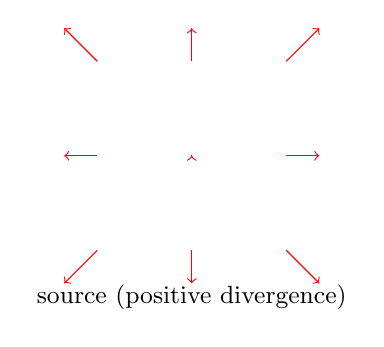
\begin{tikzpicture}[scale=1.2]
\foreach \x in {-1,0,1}{
\foreach \y in {-1,0,1}{
\draw[->,red] (\x,\y) -- ++(0.35*\x,0.35*\y);
}
}
\node at (0,-1.5) {\small source (positive divergence)};
\end{tikzpicture}
\end{center}

%------------------------------------------------
\textbf{3. Curl of a Vector Field}

For a vector field $\mathbf{F}=(F_x,F_y,F_z)$, the curl is
$$\nabla \times \mathbf{F}
=
\begin{vmatrix}
\mathbf{i} & \mathbf{j} & \mathbf{k} \\
\partial/\partial x & \partial/\partial y & \partial/\partial z \\
F_x & F_y & F_z
\end{vmatrix}.$$

\textbf{Example.} Let
$$\mathbf{F}(x,y,z)=(-y,x,0).$$
Then
$$F_x=-y,\qquad F_y=x,\qquad F_z=0.$$
Using the determinant formula,
$$\nabla\times\mathbf{F}
=
\left(
\pdv{F_z}{y}-\pdv{F_y}{z},
\pdv{F_x}{z}-\pdv{F_z}{x},
\pdv{F_y}{x}-\pdv{F_x}{y}
\right).$$
Substitute the components:
$$\nabla\times\mathbf{F}
=
\left(
\pdv{0}{y}-\pdv{x}{z},
\pdv{(-y)}{z}-\pdv{0}{x},
\pdv{x}{x}-\pdv{(-y)}{y}
\right).$$
Now compute each term:
$$\pdv{0}{y}=0,\qquad \pdv{x}{z}=0,$$
$$\pdv{(-y)}{z}=0,\qquad \pdv{0}{x}=0,$$
$$\pdv{x}{x}=1,\qquad \pdv{(-y)}{y}=-1.$$
Therefore,
$$\nabla\times\mathbf{F}
=
(0-0,\ 0-0,\ 1-(-1))
=
(0,0,2).$$

\begin{center}
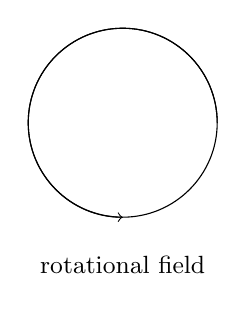
\begin{tikzpicture}[scale=1.2]
\draw[->] (0,0) circle (1);
\draw[->] (1,0) arc (0:270:1);
\node at (0,-1.5) {\small rotational field};
\end{tikzpicture}
\end{center}

%------------------------------------------------
\textbf{4. Line Integral of a Vector Field}

If a curve $C$ is parametrized by
$$\mathbf{r}(t)=(x(t),y(t),z(t)),\qquad a\le t\le b,$$
then the line integral of $\mathbf{F}$ along $C$ is
$$\int_C \mathbf{F}\cdot d\mathbf{r}
=
\int_a^b \mathbf{F}(\mathbf{r}(t))\cdot \mathbf{r}'(t)\,dt.$$

\textbf{Example.} Let
$$\mathbf{F}(x,y)=(y,x),
\qquad
\mathbf{r}(t)=(t,t^2),
\qquad 0\le t\le 1.$$
First compute the derivative of the parametrization:
$$\mathbf{r}'(t)=\left(\dv{t}t,\dv{t}(t^2)\right)=(1,2t).$$
Now substitute the curve into the vector field:
$$\mathbf{F}(\mathbf{r}(t))
=
\mathbf{F}(t,t^2)
=
(t^2,t).$$
Now compute the dot product:
$$\mathbf{F}(\mathbf{r}(t))\cdot \mathbf{r}'(t)
=
(t^2,t)\cdot(1,2t)
=
t^2\cdot 1+t\cdot 2t
=
t^2+2t^2
=
3t^2.$$
So the line integral becomes
$$\int_C \mathbf{F}\cdot d\mathbf{r}
=
\int_0^1 3t^2\,dt.$$
Now integrate:
$$\int_0^1 3t^2\,dt
=
3\int_0^1 t^2\,dt
=
3\left[\frac{t^3}{3}\right]_0^1
=
[t^3]_0^1
=
1-0
=
1.$$
Therefore,
$$\int_C \mathbf{F}\cdot d\mathbf{r}=1.$$

\begin{center}
\begin{tikzpicture}[scale=1.2]
\draw[->] (-0.5,0) -- (2.5,0);
\draw[->] (0,-0.5) -- (0,3);
\draw[thick] plot[domain=0:1.4,samples=50] (\x,{\x*\x});
\draw[->,blue] (0.8,0.64) -- (1.1,1.0);
\node at (1.7,2.5) {\small curve $C$};
\end{tikzpicture}
\end{center}

%------------------------------------------------
\textbf{5. Stokes' Theorem}

Let $S$ be an oriented smooth surface with positively oriented boundary $\partial S$. Then
$$\oint_{\partial S}\mathbf{F}\cdot d\mathbf{r}
=
\iint_S (\nabla\times\mathbf{F})\cdot \mathbf{n}\,dS.$$

\textbf{Example.} Let
$$\mathbf{F}(x,y,z)=(-y,x,0),$$
and let $S$ be the unit disk in the plane $z=0$, oriented upward.

From the previous computation,
$$\nabla\times\mathbf{F}=(0,0,2).$$
The upward unit normal vector is
$$\mathbf{n}=(0,0,1).$$
Thus,
$$(\nabla\times\mathbf{F})\cdot\mathbf{n}
=
(0,0,2)\cdot(0,0,1)=2.$$
So the surface integral is
$$\iint_S (\nabla\times\mathbf{F})\cdot \mathbf{n}\,dS
=
\iint_S 2\,dS
=
2\iint_S dS.$$
Since $S$ is the unit disk, its area is $\pi$, therefore
$$\iint_S (\nabla\times\mathbf{F})\cdot \mathbf{n}\,dS
=
2\pi.$$

Now compute the line integral around the boundary circle $\partial S$:
$$\mathbf{r}(t)=(\cos t,\sin t,0),\qquad 0\le t\le 2\pi.$$
Then
$$\mathbf{r}'(t)=(-\sin t,\cos t,0).$$
Substitute the curve into the field:
$$\mathbf{F}(\mathbf{r}(t))
=
(-\sin t,\cos t,0).$$
Now compute the dot product:
$$\mathbf{F}(\mathbf{r}(t))\cdot \mathbf{r}'(t)
=
(-\sin t,\cos t,0)\cdot(-\sin t,\cos t,0)
=
\sin^2 t+\cos^2 t
=
1.$$
Thus,
$$\oint_{\partial S}\mathbf{F}\cdot d\mathbf{r}
=
\int_0^{2\pi}1\,dt
=
[t]_0^{2\pi}
=
2\pi.$$
Hence
$$\oint_{\partial S}\mathbf{F}\cdot d\mathbf{r}
=
\iint_S (\nabla\times\mathbf{F})\cdot \mathbf{n}\,dS
=
2\pi.$$

\begin{center}
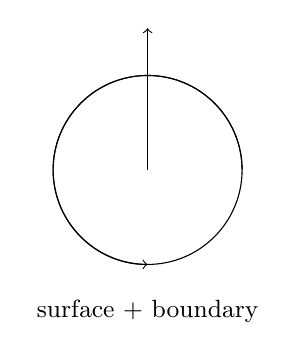
\begin{tikzpicture}[scale=1.2]
\draw (0,0) circle (1);
\draw[->] (0,0) -- (0,1.5);
\draw[->] (1,0) arc (0:270:1);
\node at (0,-1.5) {\small surface + boundary};
\end{tikzpicture}
\end{center}

%------------------------------------------------
\textbf{6. Gauss--Ostrogradsky Theorem (Divergence Theorem)}

Let $V$ be a solid region with closed boundary surface $\partial V$ and outward unit normal vector $\mathbf{n}$. Then
$$\iiint_V (\nabla\cdot\mathbf{F})\,dV
=
\iint_{\partial V}\mathbf{F}\cdot\mathbf{n}\,dS.$$

\textbf{Example.} Let
$$\mathbf{F}(x,y,z)=(x,y,z),$$
and let $V$ be the unit ball
$$x^2+y^2+z^2\le 1.$$

First compute the divergence:
$$\nabla\cdot\mathbf{F}
=
\pdv{x}{x}+\pdv{y}{y}+\pdv{z}{z}
=
1+1+1
=
3.$$
Therefore,
$$\iiint_V (\nabla\cdot\mathbf{F})\,dV
=
\iiint_V 3\,dV
=
3\iiint_V dV
=
3\cdot \operatorname{Vol}(V).$$
The volume of the unit ball is
$$\operatorname{Vol}(V)=\frac{4\pi}{3}.$$
Hence
$$\iiint_V (\nabla\cdot\mathbf{F})\,dV
=
3\cdot\frac{4\pi}{3}
=
4\pi.$$

Now compute the flux through the boundary sphere $\partial V$.

On the unit sphere, the outward unit normal vector is
$$\mathbf{n}=(x,y,z),$$
because every radius vector has length $1$ there.
Also,
$$\mathbf{F}(x,y,z)=(x,y,z).$$
So
$$\mathbf{F}\cdot\mathbf{n}
=
(x,y,z)\cdot(x,y,z)
=
x^2+y^2+z^2.$$
On the unit sphere,
$$x^2+y^2+z^2=1,$$
therefore
$$\mathbf{F}\cdot\mathbf{n}=1.$$
Thus the surface integral becomes
$$\iint_{\partial V}\mathbf{F}\cdot\mathbf{n}\,dS
=
\iint_{\partial V}1\,dS
=
\operatorname{Area}(\partial V).$$
The area of the unit sphere is
$$\operatorname{Area}(\partial V)=4\pi.$$
Hence
$$\iint_{\partial V}\mathbf{F}\cdot\mathbf{n}\,dS=4\pi.$$

So both sides are equal:
$$\iiint_V (\nabla\cdot\mathbf{F})\,dV
=
\iint_{\partial V}\mathbf{F}\cdot\mathbf{n}\,dS
=
4\pi.$$

\begin{center}
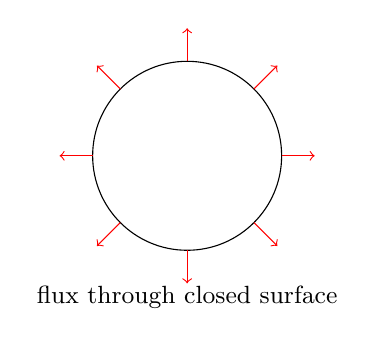
\begin{tikzpicture}[scale=1.2]
\draw (0,0) circle (1);
\foreach \a in {0,45,...,315}{
\draw[->,red] ({cos(\a)}, {sin(\a)}) -- ({1.35*cos(\a)}, {1.35*sin(\a)});
}
\node at (0,-1.5) {\small flux through closed surface};
\end{tikzpicture}
\end{center}

\end{document}

% ---------------------------------------------------------------------

